\documentclass[border=10pt]{standalone}
\usepackage{tikz}
\usetikzlibrary{arrows.meta, shapes, calc}

\begin{document}
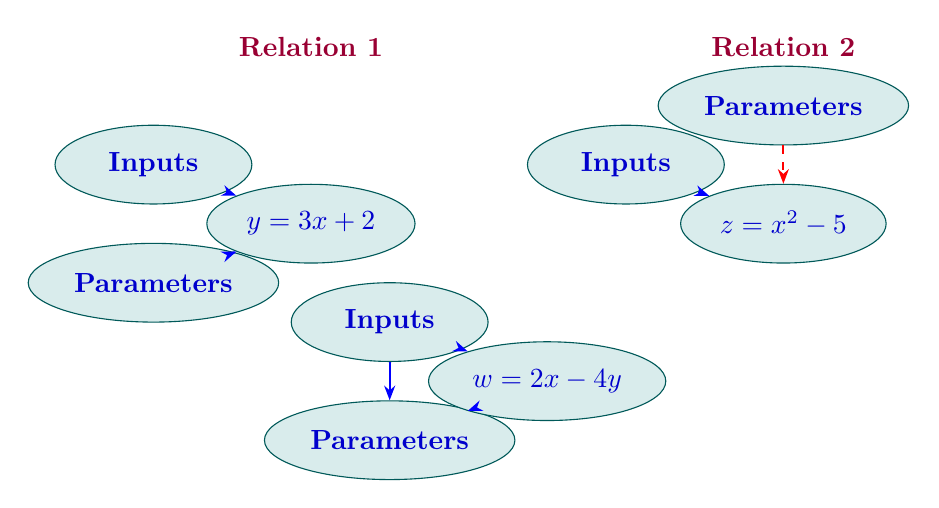
\begin{tikzpicture}[
    node distance=1.5cm,
    oval/.style={ellipse, draw=teal!70!black, fill=teal!15, minimum width=2.5cm, minimum height=1cm, font=\bfseries\color{blue!80!black}},
    title/.style={font=\bfseries\color{purple!80!black}, text width=3cm, align=center},
    arrow/.style={thick, -{Stealth[scale=0.8]}, blue},
    dashed_arrow/.style={thick, dashed, -{Stealth[scale=0.8]}, red}
]

% Relation 1
\node[title] at (0, 3.5) {Relation 1};
\node[oval] (R1_inputs) at (-2, 2) {Inputs};
\node[oval] (R1_params) at (-2, 0.5) {Parameters};
\node[oval] (R1_eq) at (0, 1.25) {$y = 3x + 2$};

\draw[arrow] (R1_inputs) -- (R1_eq);
\draw[arrow] (R1_params) -- (R1_eq);

% Relation 2
\node[title] at (6, 3.5) {Relation 2};
\node[oval] (R2_inputs) at (4, 2) {Inputs};
\node[oval] (R2_params) at (6, 2.75) {Parameters};
\node[oval] (R2_eq) at (6, 1.25) {$z = x^2 - 5$};

\draw[arrow] (R2_inputs) -- (R2_eq);
\draw[dashed_arrow] (R2_params) -- (R2_eq);

% Relation 3
\node[title] at (3, -0.5) {Relation 3};
\node[oval] (R3_inputs) at (1, 0) {Inputs};
\node[oval] (R3_params) at (1, -1.5) {Parameters};
\node[oval] (R3_eq) at (3, -0.75) {$w = 2x - 4y$};

\draw[arrow] (R3_inputs) -- (R3_eq);
\draw[arrow] (R3_params) -- (R3_eq);
\draw[arrow] (R3_inputs) -- (R3_params);

\end{tikzpicture}
\end{document}